% Name: A shift in demand
% Description: Demand moving right from D₁ to D₂ along a fixed supply curve, which raises both the equilibrium price and the quantity.
% Tags: demand shift, comparative statics, equilibrium, supply and demand

\usetikzlibrary{arrows.meta}

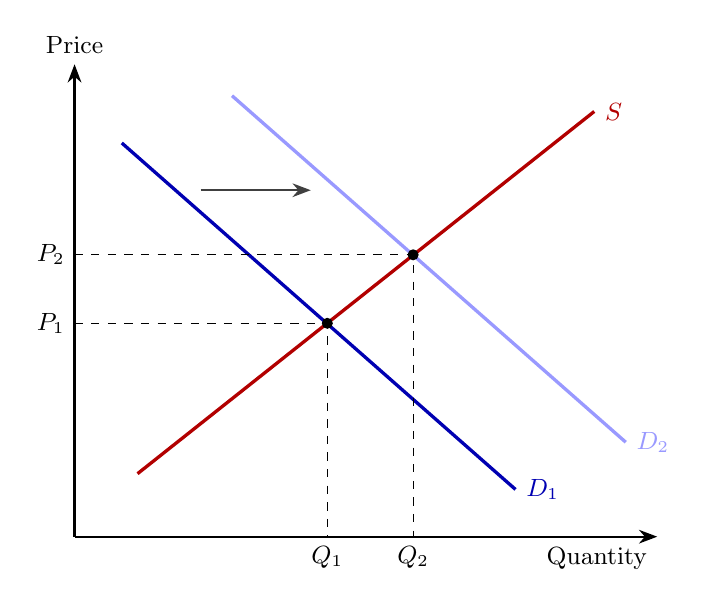
\begin{tikzpicture}[every node/.style={font=\small}, >={Stealth}]
  \draw[->, thick] (0,0) -- (7.4,0) node[below left] {Quantity};
  \draw[->, thick] (0,0) -- (0,6) node[above] {Price};
  \draw[very thick, red!70!black] (0.8,0.8) -- (6.6,5.4) node[right] {$S$};
  \draw[very thick, blue!70!black] (0.6,5) -- (5.6,0.6) node[right] {$D_1$};
  \draw[very thick, blue!40] (2,5.6) -- (7,1.2) node[right] {$D_2$};
  \draw[->, thick, gray!50!black] (1.6,4.4) -- (3,4.4);
  % Where each demand curve meets supply.
  \draw[dashed] (0,2.71) node[left] {$P_1$} -| (3.21,0) node[below] {$Q_1$};
  \draw[dashed] (0,3.58) node[left] {$P_2$} -| (4.3,0) node[below] {$Q_2$};
  \fill (3.21,2.71) circle (2pt);
  \fill (4.3,3.58) circle (2pt);
\end{tikzpicture}
